%\chapter{Integrating the Weather Model into the Sailing Path Generation}
% Question to answers during the next chapters
%%% Instruments used, set-up, materials
%%Description of the instruments and materials
%%How the instruments are set-up and what auxiliary connections might need to be used.
% How does the wind model at different time steps is going to be integrated?
%What mathematical approach is going to be use for the problem?
%How many control points define the route ? why?
%Which solver, software or algorithm is going to be use?
%How is defined the optimization problem?
% Analysis Questions
%What were the changes in the route due to the step time change?
%What is the shape of the area considered? Set-Up
%The manoeuvres/turn  jargon and conditions are represented on the model?

\chapter{The Weather Research and Forecasting Model(WRF) in the Sailing Path Generation} \label{ch:weatherModel} %The Weather Model and the Generation of the Sailing Path

%Introduction
The wind model used in this research is a numerical weather prediction (\acrshort{nwp}) knows as the Weather Research and Forecasting Model (\acrshort{wrf}). This particular model has the ability to forecast weather and serves as a tool for atmospheric research.  
This chapter explains the characteristics of the common weather forecast provided during and before the Olympic sailing races and compared it with the requirements of athletes and coaches. This comparison shows the importance of a customize weather(wind) model and describes its characteristics and limitations. \par \noindent 
For the purpose of this project, the model provided is a \acrshort{wrf} wind model stored in a NetCDF file while the measured data from past race events is provided in a tabular layout. The last part of the chapter explains the reference frames and their relation with the sailboat velocity.\par
%model used in this research. 

The importance of the wind is not only because it is considered the main propulsion source of the sailboat; but also, because it is the wind that demands changes to the seamanship, like direction on the rudder and sail, to balance the kinematic equations of chapter \ref{ch:physics_sailboat}, and reach the maximum velocity  estimated by the \acrshort{vpp}.In such a manner, the seamanship uses the wind information to maximize the velocity of the sailboat by adjusting the direction of the sailboat in a similar way the algorithm for path generation uses that information. \par 

\nomenclature[A]{NWP}{Numerical Weather Prediction}
\nomenclature[A]{WRF}{Weather Research and Forecasting Model}

%The Weather Research and Forecasting (WRF) model is a numerical weather prediction (NWP) system for forecasting weather and atmospheric research. Becuase of this duality it 


%The seamanship determine the direction of the sailboat      based on the wind direction. In the other hand, \acrshort{vpp} determines the maximum speed that the sailboat can attain at different wind velocities and directions.

\section{The application of the weather models into Olympic Sailing Races}
%WRF weather models into Olympic sailing races}

A wind model forecast is based on a 3-dimensional time-space model, which can be described as a 4-dimensional model. The resolution of this model or granularity is defined by the size of the data sets that describe it. Moreover, the use of weather models during the summer Olympic Games is not new but neither widely used. In sailing, the main use of them is as an informative source for the organizers, it helps to warranty the safety of the competitors, like in the Para-Olympic events and reduce delays due to the wind conditions of the competition  \cite{spark2004wind},\cite{sheng2009structure}, \cite{golding2014forecasting}. Only \cite{giannaros2018ultrahigh} %a couple of publications refers to these models
refers to the \acrshort{nwp} model as a tool to develop a strategic plan to course the race for a sailing team. \par 

Previous to competing athletes and coaches know the exact location of the sailing area which is enclosed by a diameter of a magnitude between 0.8 and 1.5 nm (1.482 - 2.778 km) and course diagrams \cite{SailRaceRio}. For them, it is important to identify wind patterns, like average magnitude, direction, the range of variation, the location of vortexes, and even the time of the day when they occur. This information allows the coaches and athletes to develop an strategic plan to course the race by avoiding undesirable conditions or to maximize the use of favorable zones.\par

Even when the location, dates and times of the races are known, the wind characteristic and details about the area is not well understood. The time horizons of local forecasts of short term know as \textit{nowcast} for public access is between 1 to 2 hours as a minimum and up to 6 hours, with a spatial resolution between 40 to 100 km \cite{warner2010numerical}, \cite{kristensen2010weather}. These local predictions use measurements from weather stations or any weather data available around the area of interest and extrapolate in time these conditions;
%This forecast is an extrapolation in time of known weather parameters, including those obtained by means of remote sensing, using techniques that take into account a possible evolution of the air mass
whereas days or weekly forecast can use deterministic predictions.\par
Because sailing Olympic races are set into a grid of 2km with a maximum duration of 1 hour; the public information about wind (weather forecast) does not meet the requisites of the athletes and coaches. As a consequence, customize models have to been developed for them to provide the information required. A clear example of this type of models was developed by Giannaros \cite{giannaros2018ultrahigh}, which is defined as a \acrshort{wrf} with \textit{ultrahigh resolution wind forecasting}.\par 
An ultrahigh resolution, a detailed level of granularity, means that the spatial variation captured by the model is in the order of hundred meters in the horizontal plane. In this case, the minimum grid size used was about 200 meters on the area of interest and surrounded by different grid sizes up to 25 km. The vertical dimension was defined by 40 unequally spaced elevations or altitudes; while the duration of the forecast stands for 48 hours starting at 0:00 UTC hours each day with a time interval or time step of 30 minutes. \par \noindent 
Just considering the area of the course which is placed within a grid of 2 km, a model of ultrahigh resolution has a granularity of 10,200 data sets or 39.5$\times 10^6$ data points. The model developed by Giannaros has more data sets since the \acrshort{nwp} model considers a larger area around the races and other factors which will be explained in the next section. Furthermore, it
%The total number of points for a course placed on a grid of 2km is around 39.5$\times 10^6$  data sets assuming and These model 
was calculated using 300 computer cores of a high-performance computing cluster and more than 900,000 core hours \cite{giannaros2018ultrahigh}. 

Before \cite{giannaros2018ultrahigh}, only \cite{philpott2001optimising} and \cite{allsopp2000optimal} developed models to include the weather for offshore yacht competitions. Instead of using an \acrshort{nwp} model to determine the wind, each work uses a different stochastic process to calculate it. The details about the discretization of the time were not provided. Only \cite{philpott2001optimising} acknowledge a short-course competition where the Markov process only applied to the wind direction; the granularity of the model was 4000 data sets with a time step of 5 seconds. %The Markov process used only refers to the direction of the wind.
Other applications of wind models refer to vessels routing where the focus is on fuel costs and other logistics metrics. \par 
% add conclusion of the model
The \acrshort{wrf} model can provide the detailed information required by the sailors and coaches of Olympics Classes; however, it demands time and high-performance computing equipment, without considering the preliminary input data and validation process it requires to have a feasible and reliable model to work with. In the other hand, the inclusion of weather models for path generation has not evaluated the sensibility of the trajectory due to the granularity of the model. The next section will provide the details about the \acrshort{wrf} model used for this project as well as its general characteristics. \par %of this type of models. \par % and how the findings of \cite{giannaros2018ultrahigh} related to its usage are considered.\par

\section{Components of the WRF Wind Model}
Weather models, like wind or current models, are discretized over the space and time because the data is organized into a four-dimensional grid data sets. The most used computer formats to share this type of models are GRIB(.grib) and NETCDF(.nc). The form in which they organize the information may differ but both formats contain the volume representation of the wind model. A straightforward format sometimes used to share the information is the tabular format with all the variables as headers. \par

\subsection{The WRF Model }
The \acrshort{wrf} is a model that combines global atmospheric models with regional measurements to developed high-resolution models. This means that regional models are inserted within global models, as a result, its range of applications is from meters to many latitude-longitude degrees. The integration allows the identification of small climate variations and other types of phenomena, like precipitations. The incorporation of observable data measured at a constant rate and at known locations given flexibility to the model and unification of the available data \cite{warner2010numerical}. \par

\subsection{Spatial Representation of the Wind Model}

Weather models are volume representations of a particular region because of this, it is important to identify the data dimensions, to either manipulate or extract properly the variable of interest, like the wind velocity, if the height does not match the CE of the sail, equation \ref{eq:wind_h} should be used to determine it. \par \noindent %the wind velocity. \par
Figure \ref{fig:map_projection} shows the sketches of the most common type of map projection used on atmospheric modeling. The main idea of these projections is that a set of rays coming from the same axis of rotation project points from the sphere into the surface of projection which latter can be flattened. %The Mercator map projection is base on a cylinder projection which can be make flat when it is cut. %So each point or feature on the sphere is projected on the cylinder, 
%this allows the flat representation of the sphere %however at some locations some geometrical characteristics are out of proportion. 
The advantage of them %this map representations
is that the angles between curves are preserved and the distance distortions are the same in all directions of a point. The map projection to use depends basically %used then basically depends 
on the latitude of interest \cite{warner2010numerical}. \par

\begin{figure}
    \centering
    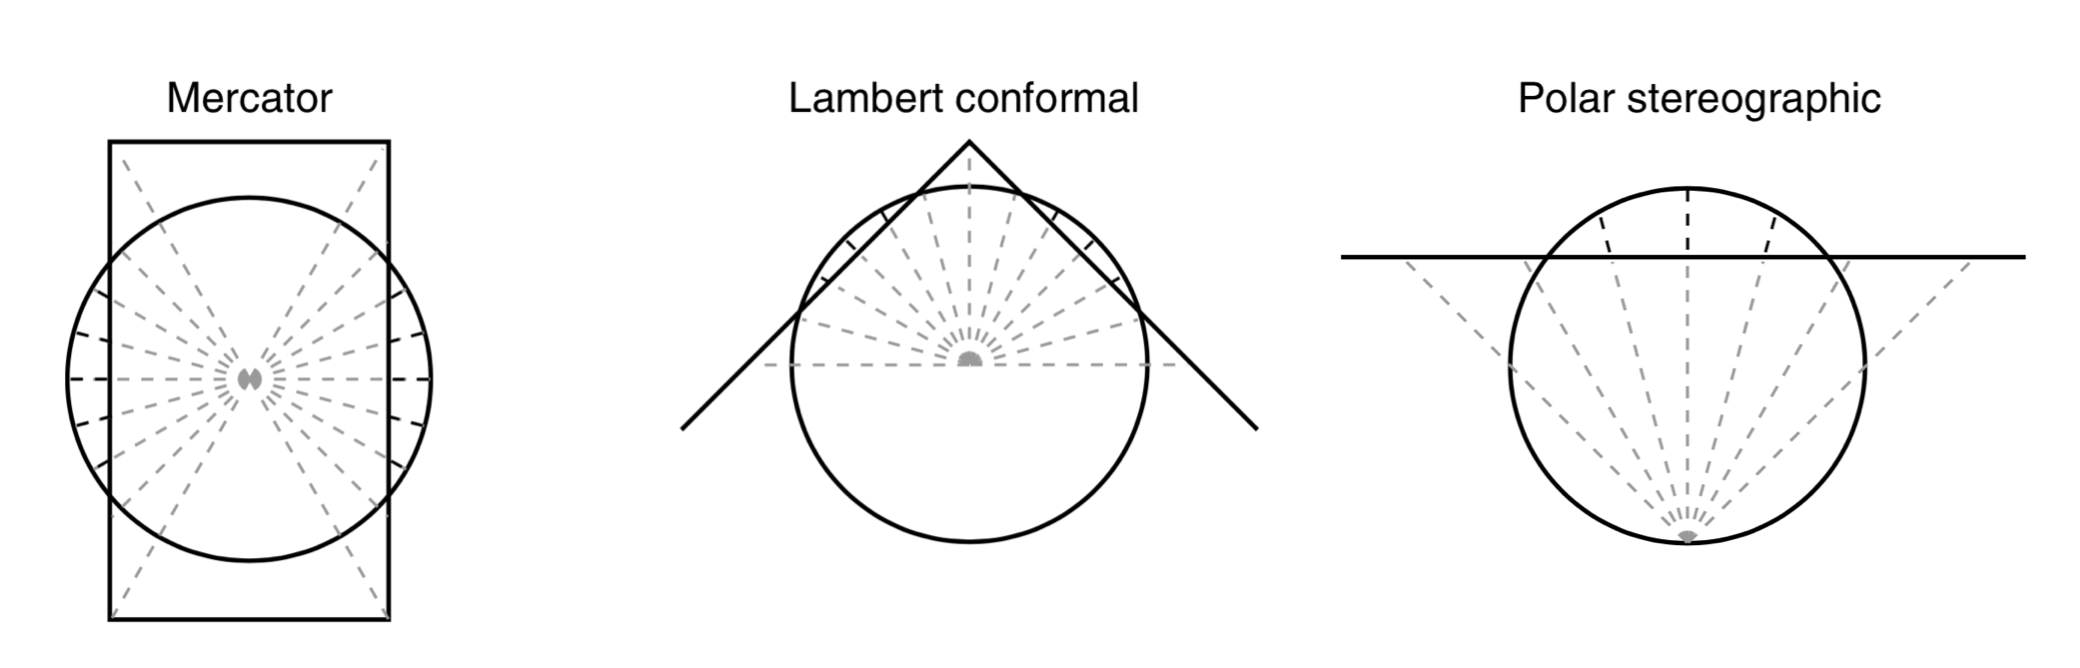
\includegraphics[width=1 \linewidth]{map_proj.png}
    \caption{Most common map projections used on atmospheric models. Mercator is a cylinder projection commonly used for grids in tropical latitudes, Lambert-conformal is a cone, used for mid-latitude grids and the Polar stereographic uses a plane and is used for high latitude grids. The axis of all 3 is always coincident with the Earth's axis. \cite{warner2010numerical}.}
    \label{fig:map_projection}
    %  The cylinder (Mercator), right-circular cone (Lambert conformal), and plane (polar stereographic) are the surfaces on which the information on the sphere is projected. The radial lines connect points on the sphere and points on the projection surface. The axes of the cylinder and the cone, and the perpendicular to the plane, are parallel to Earth’s axis of rotation. In these images, we are thus viewing Earth from over the Equator.}
\end{figure}

%The value of $\Delta x$ is chosen to have sufficient number of grid points to adequately represent the smallest meteorological feature of interest.\par 
%the truncation error quantifies the accuracy associated with representing continuous functions with a finite number of points. \par
%The numerical framework  used on the model of wind to solve the space dependence in the nonlinear partial differential equations of atmospheric dynamics and thermodynamics. 

The points on the spatial grid of the \acrshort{wrf} model are quasi-regular because the grid is defined by the map projection %of the Earth's surface 
used. Each intersection of the grid is a data point defined by 4 dimensions (\textit{$n(x_{i},y_{j},z_{k},t)$}) and it represents the location of a variable value. %, which could be either a measurement or an estimation. 
The value of $\Delta x$ is chosen to have a sufficient number of grid points to adequately represent the smallest meteorological feature of interest. \par

Under some circumstances, the model uses a nested approach; where $\Delta x$ is reduced as it gets close to the area of interest. The size of the grid was a crucial concern for \cite{giannaros2018ultrahigh} since the topography of public databases were replaced by new sets that at least match the size of the stipulated grid.\par

\subsection{Time Representation on the Wind Model}
The time dimension on the forecast models is limited by the \textit{Courant number} and in consequence with the spatial resolution required. Modifications on the grid have implications closely related with the computational effort; since on each time step the space equations on each grids point, have to be solved. The measurement data is another element to incorporate and related to time. \par 

The computational effort for weather models results from the space granularity. Meanwhile, the time step brings stability to the model. Then a small time step provides stable solutions to the equations. 
%The time steps are smaller con satisfy the stability condition.\par
While the computational effort is related to the space granularity in a non-linear form. For example, if only one space dimension is double (by a factor of 2), the computational effort time will be 8 times more. \par 
% increasing one space dimension by a factor of 2 results in a factor of 8 in the computational effort time it takes to solve the model. \par %an increase of the computational time by a factor of 8. \par
The use of measurement data has an impact on the quality of the results because the rate of their incorporation and values adjust the model forecast. Figure \ref{fig:data_meas_integration} shows how often the measured data is incorporated into the model. This incorporation determines the rate of the re-initialize and the number of cycles %ation 
within the model forecast that it has to assimilate the observable values. %This %rate 
%defines the number of cycles %within the forecast %that the model has to re-run 
%This merge and assimilate the new values. 
In this form, the measured data %. In this form, the merge of cycles or assimilation process %of measured data 
not only affects the time of processing but also the accuracy of the forecast. \par %, without it the model performs interpolation
\begin{figure}
    \centering
    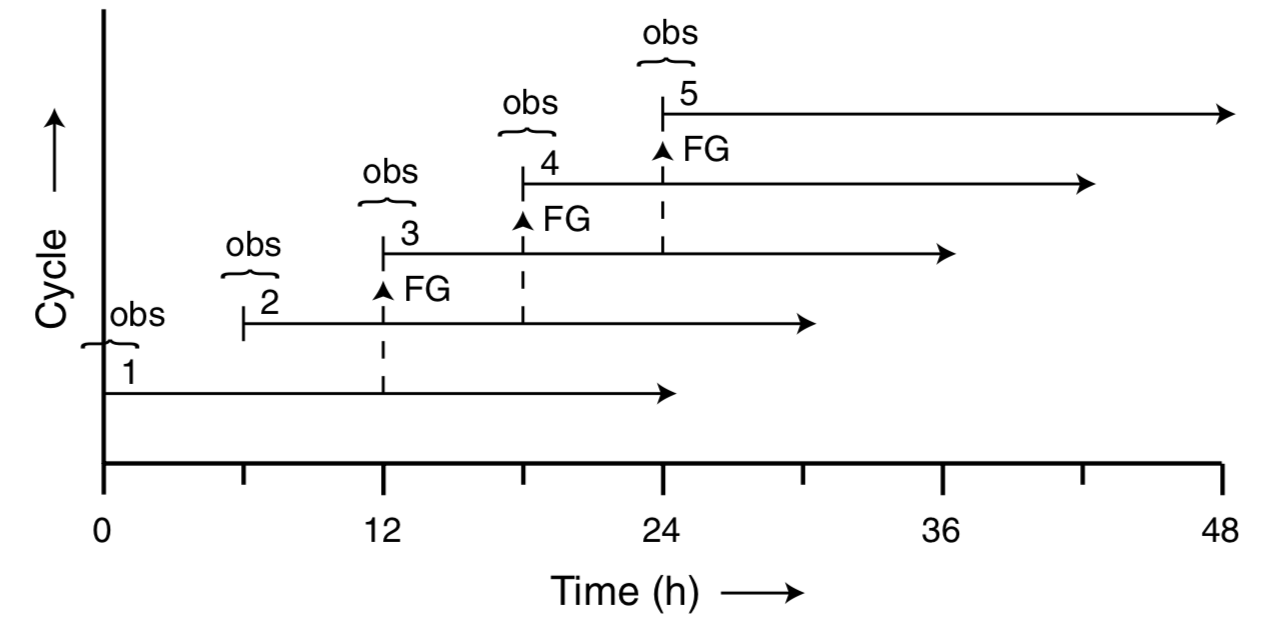
\includegraphics[width=1 \linewidth]{re-run_model.png}
    \caption{Forecast Model with the integration of measured data. During 24 hours, the forecast models is adjusted every 6 hr by the observations. This generates 4 cycles which are assimilated by the model \cite{warner2010numerical}. }
    \label{fig:data_meas_integration}
\end{figure}

\section{The WRF model for the World Cup Series 2018 Hyéres, France}

The algorithm for the minimal time path for sailing competitions was developed considering the characteristics of the \acrshort{wrf} wind model on a date of competitions so wind measurements are available. The measurements served not only to set-up the model but also to compare their results. Since \cite{giannaros2018ultrahigh} found that the topography allocation and representation in addition to the initialization of the model have a great impact on the results. \par

The World Cup Series 2018 Hyéres, France Laser competition was chosen. The area where the races took place was named as Charly and the coordinates of its center were: 43\degree 02.869'N, 006\degree 13.221' E. The diameter of the area was 1.6 nm (2.96 km). The date was April 24, 2018. The model forecast 24 hours starting at 0:00 Hrs local time and it was provided by professor Sukanta Basu from the Geoscience Department at TU Delft. \par 

The information of the wind model was stored in the NetCDF file which is organized in dimensions, variables and attributes defined as data sets \cite{netcdf56302}. In this case, 4 coordinates describe the location and time of %different variables, in this case
the wind velocity. The attributes vector refer to the dimensions of each variable, in this case, the velocity's units were $m \backslash s $. \par 

The wind speed variables were \textit{u} and \textit{v} velocities. Over a rectangle area of coordinates: 41.663\degree N, 4.752\degree E and 7.251\degree N, 44.451\degree E. The grid size is about 1 km or approx 0.009\degree. The coordinates latitude and longitude where store independently and discretize over a plane of 198$\times$300 elements. \par 
The components of the wind velocity were stored on a grid plane of 199$\times$300 for \textit{u} and 198$\times$301 for \textit{v} velocity. This arrangement is known as grid staggering where the different dependent variables are on different grids so the spatial resolution is increasing while the effects of truncation error are decreased. The velocity corresponding to each coordinate is the horizontal average velocity calculated as equations \ref{eq:hor_AVG_velu} and \ref{eq:hor_AVG_velv} indicate.  \par  %This technique to increase the spatial resolution and decreasing the effects of truncation error on the solution.  

\begin{equation} \label{eq:hor_AVG_velu}
    u_{{i,j}_{avg}}=\frac{ u_{i,j} + u_{{i+1},j} } {2}
\end{equation}

\begin{equation} \label{eq:hor_AVG_velv}
    v_{{i,j}_{avg}}=\frac{ v_{i,j} + v_{i,{j+1}} } {2}
\end{equation}

The vertical dimension, height, of the model where discretized over 50 non-uniform steps. The first level corresponds to 7.8 m while the second height is at 25 m. Because the \acrshort{ce} is estimated to be at 2.68 m from the water level \cite{pennanen2015optimal} and the measurements were taken at 10 m above the sea level, equation \ref{eq:wind_h} is used to determine the \acrshort{kappa} value and convert \acrshort{u} and \acrshort{v} fields to the corresponding height. Finally, \acrshort{v_tw} and \acrshort{b_tw} on each grid point can be calculated with equations \ref{eq:v_tw} and \ref{eq:b_tw}, respectively. \par \noindent Equation \ref{eq:b_tw} uses the four-quadrant inverse tangent, (atan2(Y,X)) from \acrshort{matlab} to return values over the [$- \pi, \pi  $] interval.% values in the closed interval [-pi,pi] based on the values of Y and X as shown in the graphic. \par

\begin{equation}\label{eq:v_tw}
    V_{tw_{i,j}}=\sqrt{{u_{i,j}}^2+{v_{i,j}}^2}
\end{equation}

\begin{equation}\label{eq:b_tw}
    \beta_{tw_{i,j}}= atan2 \frac {v_{i,j}}{u_{i,j}}
\end{equation}

The 24 hrs forecast model was discretized in time steps of 10 minutes or ${1} \backslash {6}$ hr. This means that there are 145 steps on the time dimension. Figure \ref{fig:wind_model_FR} shows the wind model provided at 2 different hours, the difference of time is only 1 hour and 10 minutes. The red cross is the center of laser course area named Charly and the black arrows indicate the direction of the wind. The figure also shows the relevance on the scale or granularity; on one side public forecast weather are larger than the one showed here; in the other hand, the interested region is too small even when the granularity was increased significantly. \par    
%the magnitude of the wind velocity ($V_{tw}$) and its direction $\beta_{tw}$

%each in a v meaning that the horizontal plane was discretize over 198x300 grid elements.  Because the time steps 145 

%The spatial resolution of the model used for the purposes of this research is a 
\begin{figure} [hb!]
  \centering
  \subfloat[Wind model forecast at 10:00 Hrs]{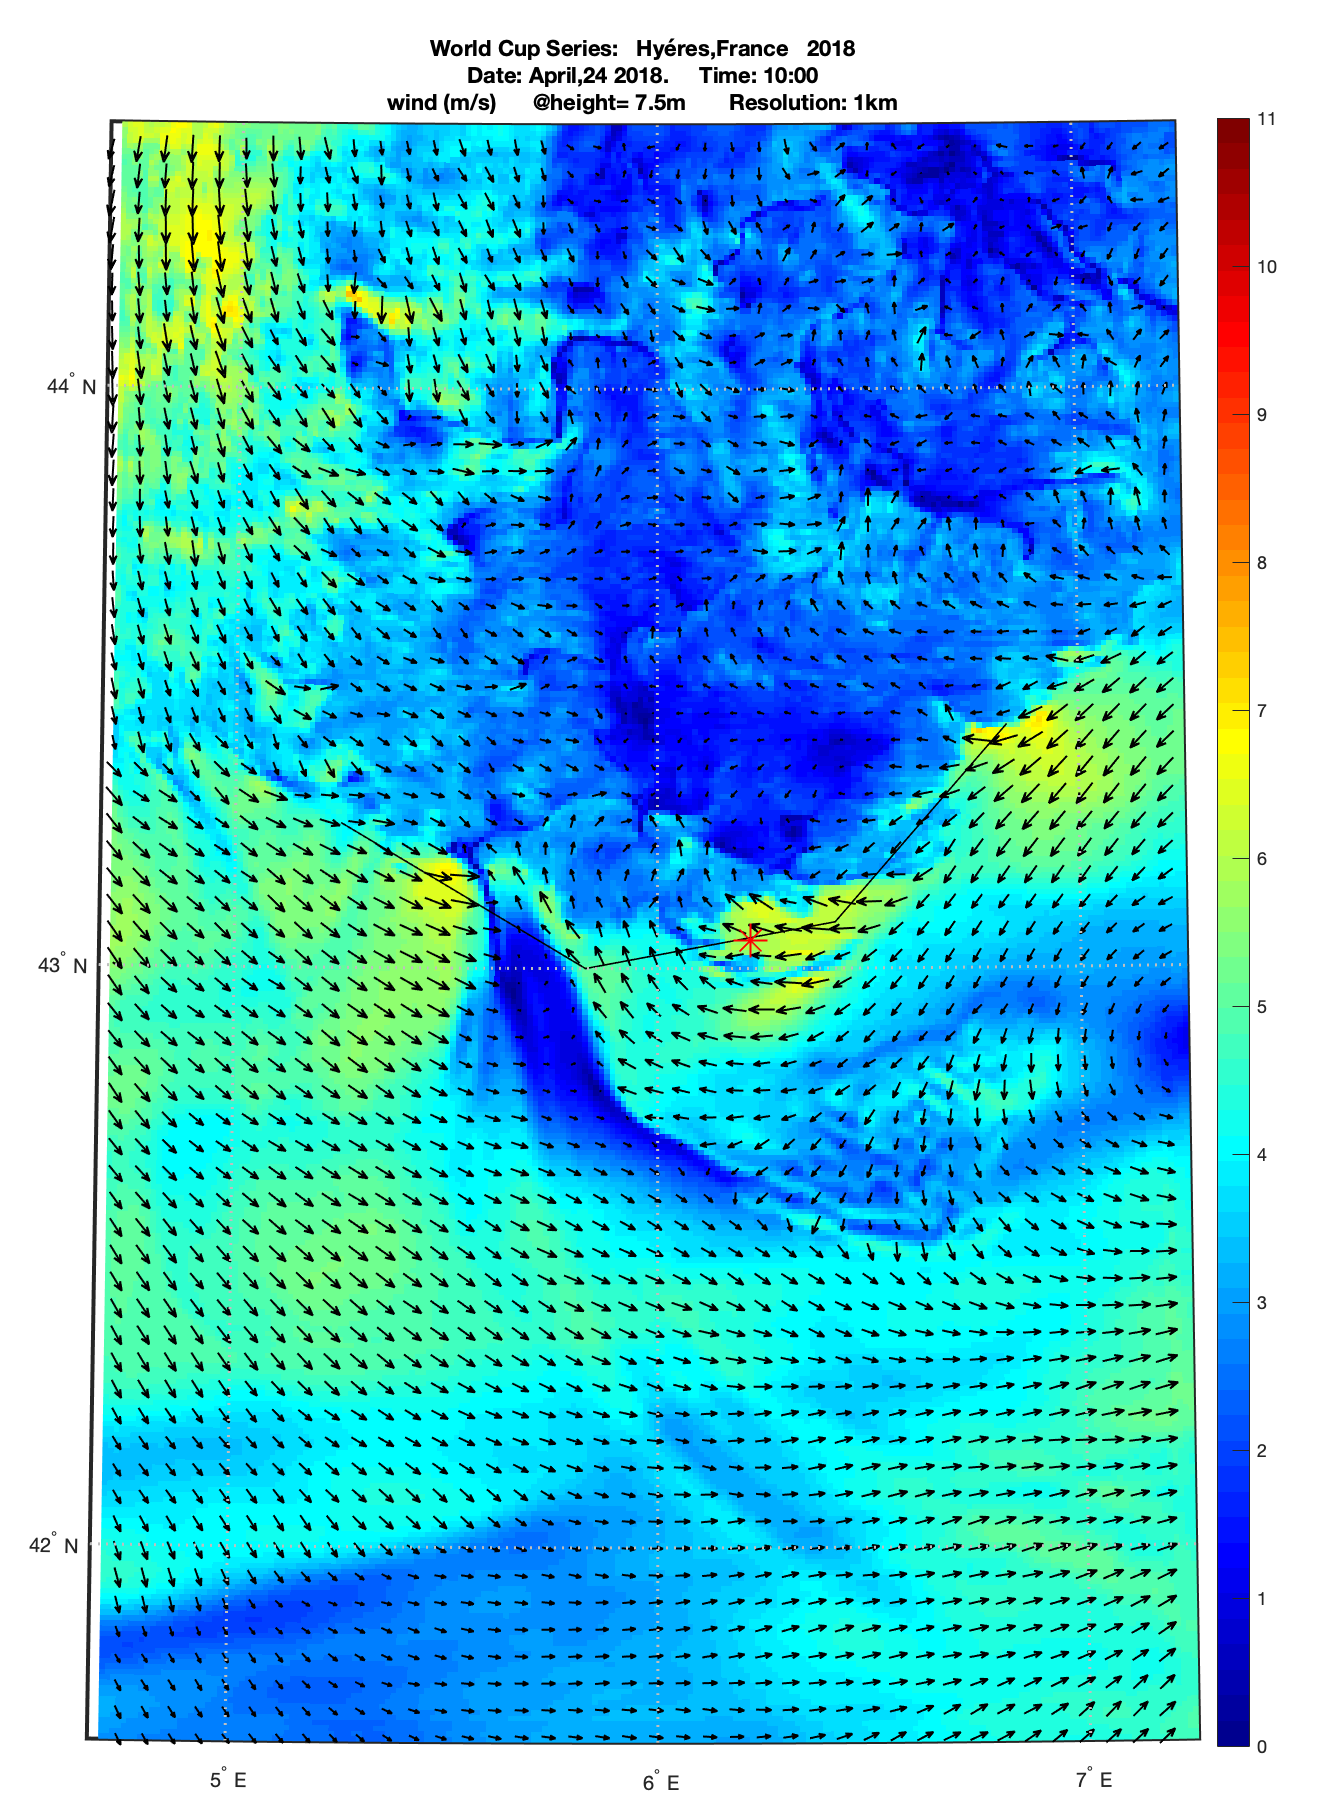
\includegraphics[width=0.5\hsize]{images/fr_10_22.png}\label{fig:fr_10hr}}
  %\hfill linewidth
  \subfloat[Wind model forecast at 11:10 Hrs]{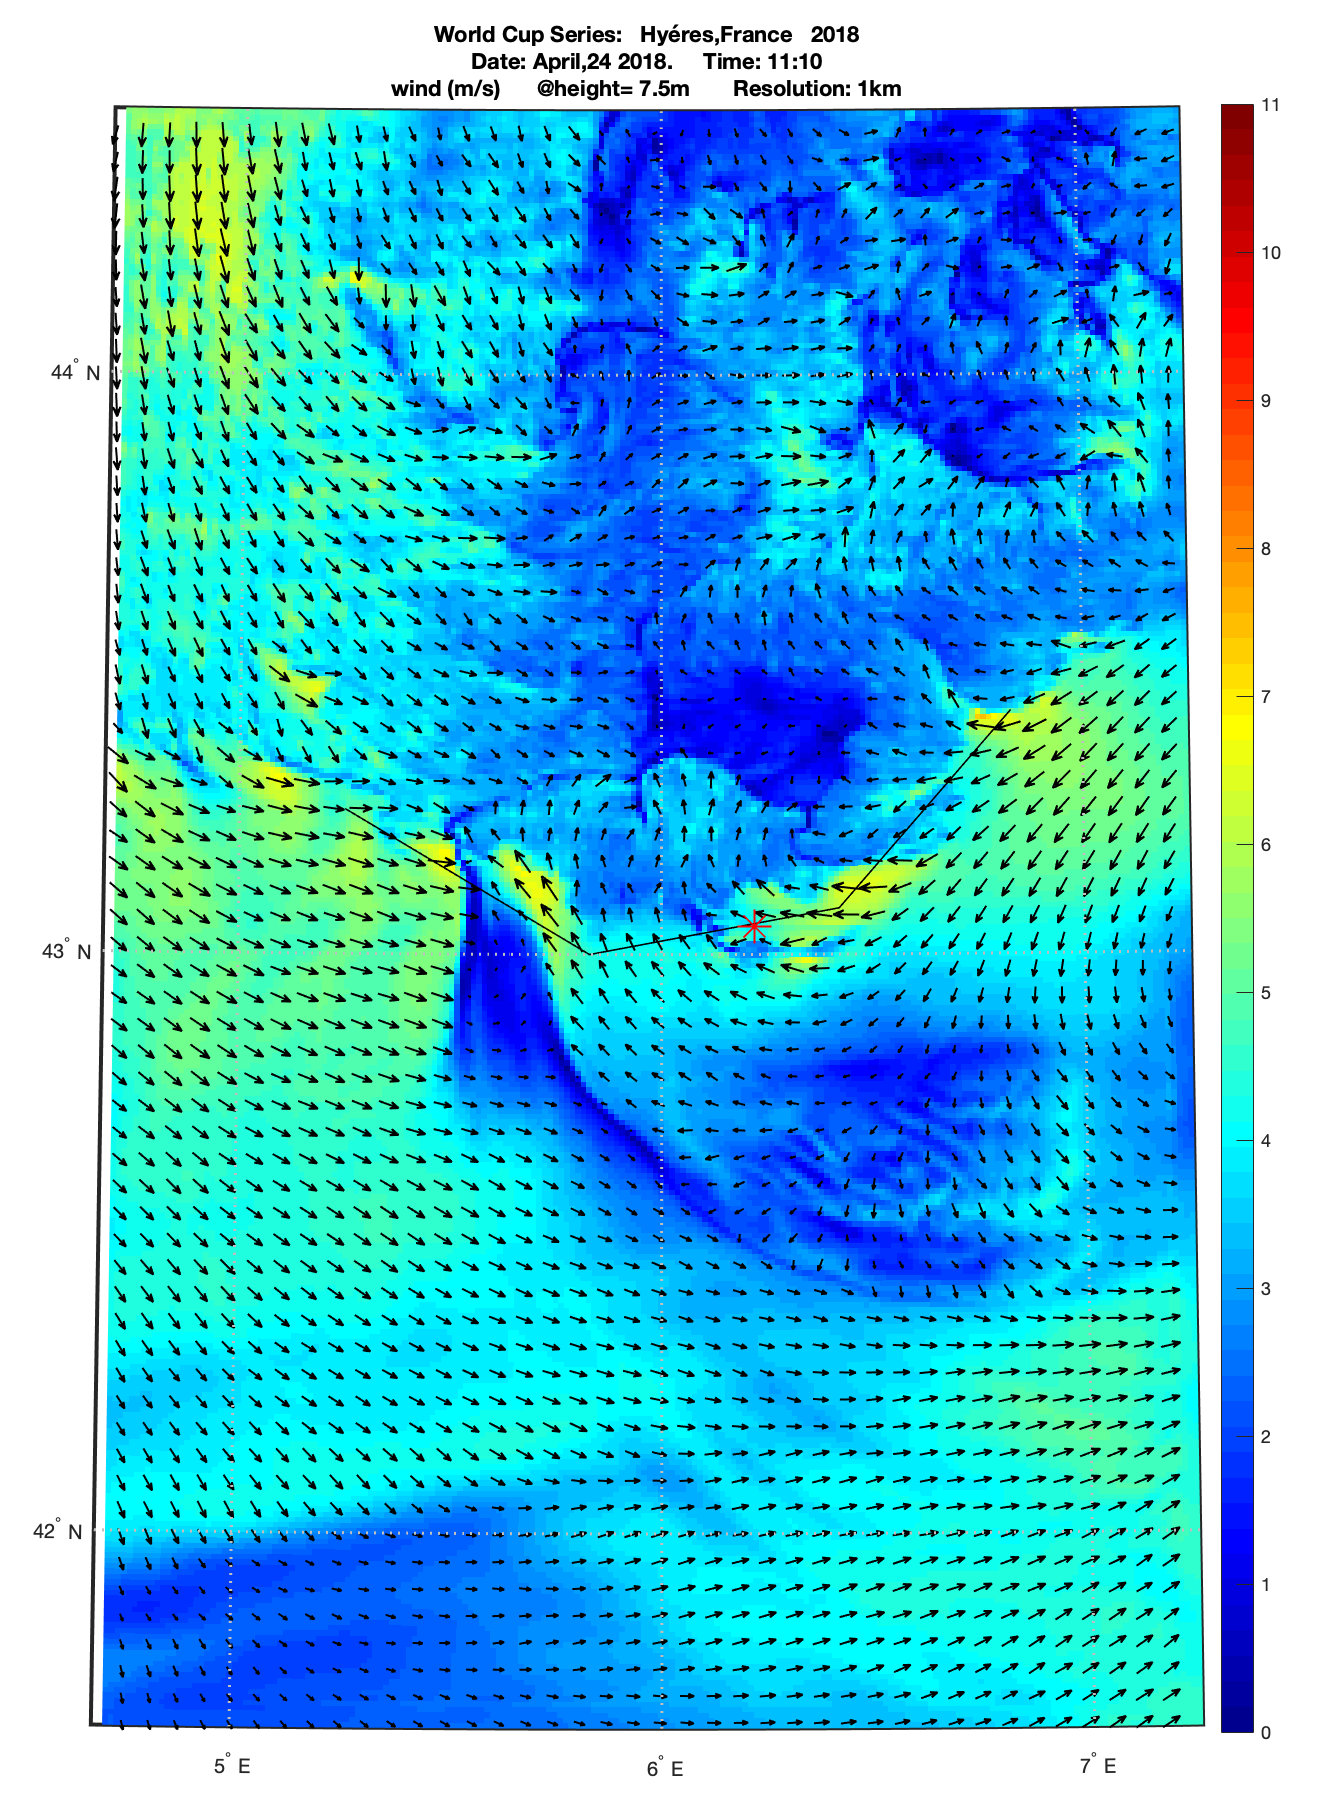
\includegraphics[width=0.5\hsize]{images/fr_11_22.png}\label{fig:fr_11hr}}
  \caption{Wind Model for the World Cup Series 2018 at Hyéres, France. The red asterisk indicated the center of the Charly area for the Laser Course. The area of the model is defined by the corner coordinates at 41.663\degree N, 4.752\degree E and 7.251\degree N, 44.451\degree E.}
\label{fig:wind_model_FR} 
\end{figure}
In resume the wind model provided is a 4D(\textit{(x,y,z,t)}) grid model of 198 $\times$ 301 $\times$ 50 $\times$ 145 datasets with a space resolution ($\Delta x$) of 1 km and time step ($\Delta t$) of 10 minutes(600 seconds). This kind of granularity is defined as high resolution, and despite the size of the grid the area of competition, its center looks small. This is one of the reasons why \cite{giannaros2018ultrahigh} developed a model with ultrahigh space resolution.\par  

\section{Reference Frames the relation between wind and sailboat velocities}

The wind velocity and direction determines the velocity of the sailboat. However, the wind velocity perceived by the seamanship when the sailboat moves is not the same as the velocity of the sailboat. This perceived velocity is known as the \textit{apparent wind} (\acrshort{v_aw}) and it not only includes the velocity and direction of the wind but also the velocity and direction of the current (\acrshort{v_tc} and \acrshort{b_tc}). The \acrshort{v_aw} and \acrshort{b_aw} are not new concepts, they were introduced on section \ref{sec:wind_vel_trian} and on equation \ref{eq:vel_appVector}. \par

The \acrshort{v_aw} is modified by the current in a similar form as on equation \ref{eq:vel_appVector}, from this equation the current vector is subtracted as shown in equation \ref{eq:vel_wind_current} this velocity is defined as \acrshort{v_awc}. The vector expression shows how different directions influence the results even when the magnitude is the same. In the other hand, if the boat is moving in the same direction as the wind then the apparent velocity increase \cite{denny2009float},\cite{allsopp1998stochastic}. \par 
%The wind velocity felt by the moving boat is w'=v-tw - v-boat.  the boat moves through the wind and so feel a wind velocity that depends on its own speed and direction 
%angle between the boat velocity and v-tw is a-vw. 

\begin{equation} \label{eq:vel_wind_current}
\vv{V_{a_{w,c}}}= \vv{V_{tw}} -\vv{V_{tc}} - \vv{V_{boat}}
\end{equation}

However, the previous equation is not the only modification to consider related to wind. %The wind model describes the velocity of the wind 
The wind model only applies over a specific region on the Earth-fixed frame, while the sailboat frame moves along it and is located as indicated by section \ref{sec:eq_of_motion}. It was assumed that the area and the trajectory of the sailboat can be expressed as [\textit{X,Y}] coordinates. This is possible for Olympic Sailing Races because the course area is relative small compared with the total surface of the Earth. Thus to convert the latitude-longitude to [\textit{X, Y}] coordinates, the \acrshort{matlab} function \textit{deg2utm(Lat, Lon)} can be used \cite{allsopp1998stochastic}.\par 
%the Earth is assumed as a \textit{great circle}; which is the circle made by the intersection of a plane over the sphere. 
\noindent For the purposes of this research, it is assumed that the Earth circumference is about 40003.2 km. In addition, the nautical mile is one minute (\textit{$1 \backslash 60 \degree$}) of arc on the surface of this sphere, thus the nautical miles is 1852 m. \par 
% A \acrshort{matlab} function used for this conversion is \textit{deg2utm(Lat,Lon)} function. \par   
\begin{figure}[hbt!]
    \centering
    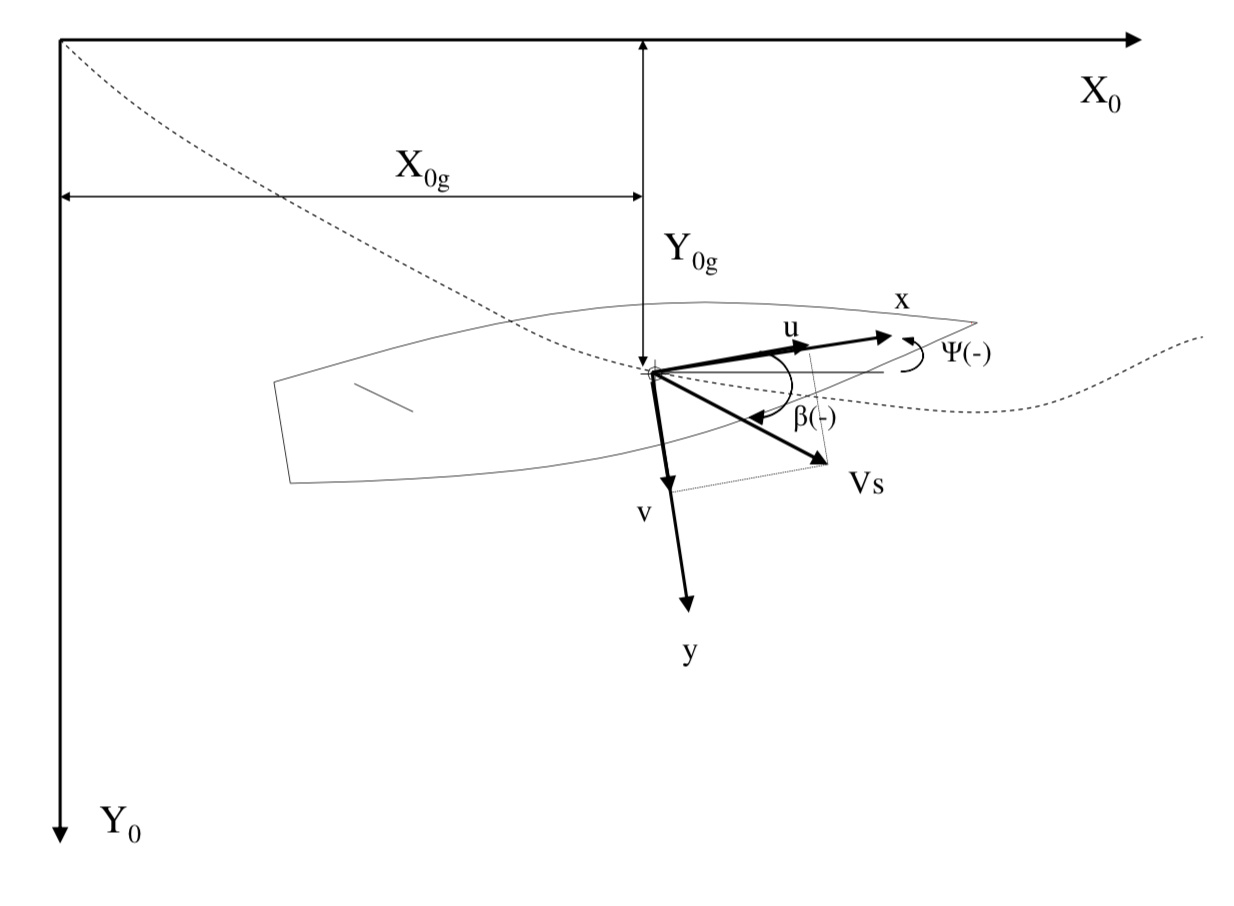
\includegraphics[width=.85 \hsize]{boat_csys.png}
    \caption{Sailboat reference coordinate system and Earth-fixed reference frame \cite{keuning2004mathematical}. }
    \label{fig:boat_Csys}
\end{figure}
Since the sailboat displaces through the horizontal plane of the wind model, another transformation has to apply in order to describe the motion and forces of the sailboat. Figure \ref{fig:boat_Csys} shows how \acrshort{u} is always aligned with the sailboat mid-plane therefore to its heading direction (-$\Psi$). The change in orientation respect to the same reference frame is done with the rotation matrix \ref{eq:RotMat}. This transformation is shown in equation \ref{eq:velTransFrame} and it expresses the velocity from the Earth-fixed frame to the sailboat-fixed frame \acrshort{v_btw} \cite{yang2011control}, \cite{bohm2014velocity}, \cite{Alves2014ASailboat}, \cite{keuning2004mathematical}.\par 
\begin{equation}\label{eq:velTransFrame}
    V_{tw}^b= \mathcal{R} \dot V_{tw}= \mathcal{R}
    \begin{bmatrix}
    u\\
    v
    \end{bmatrix}
\end{equation}

\begin{equation} \label{eq:RotMat}
    \mathcal{R}(- \Psi)=
    \begin{bmatrix}
    cos \Psi & sin\Psi \\
    -sin \Psi & cos \Psi
    \end{bmatrix}
\end{equation}

%The motion of a rigid body in space can be described by the displacement of the centre of mass of the rigid body plus the change in orientation of the rigid body with respect to some reference system, see
If the \acrshort{v_tc} is included in the model without waving effects the \acrshort{v_tw} has to be modified before the transformation of equation \ref{eq:velTransFrame}. This is expressed in equation \ref{eq:V_twModifV_C} \cite{allsopp1998stochastic}. However more equations like the \acrshort{b_aw} and \acrshort{v_aw} have to be redefined because of this inclusion. The equations modified are shown next:\par
\begin{equation}\label{eq:V_twModifV_C}
    \vv{V_{tw,c}}=\vv{V_{tw}}- \vv{V_{tc}}
\end{equation}

\begin{equation}\label{eq:v_twCurBoat}
    V_{tw,c}^b=\mathcal{R} \dot V_{tw,c}
\end{equation}

\begin{equation} \label{eq:VelCurrWind_boat}
    \vv{V_{aw,c}^b}= \vv{V_{tw,c}^b} - \vv{V_{boat}}
\end{equation}

\begin{equation}\label{eq:b_tw_c}
    \beta_{aw,c}= atan2 \frac {v_{aw,c}^b}{u_{aw,c}^b}
\end{equation}

The transformation of the terms from the sailboat-fixed to the Earth-fixed coordinate system and \acrshort{v_tw} using \acrshort{RM} is not necessary on the equations from \ref{sec:eq_of_motion} since they were already included in their development \cite{keuning2004mathematical}.\par  
%the transformation of the added mass terms from the body fixed to the earth fixed coordinate system is no longer necessary because we now approximate the added mass of the asymmetric sections of the heeled yacht in the horizontal plane directly. 

%Both coordinate systems have their x-axes in the direction of motion of the yacht, but one is always upright while the other one heels with the boat having its xy-plane always perpendicular to the mast if the mast is positioned straight on the boat with no forward or aft rake.

%$V_{aw}$ and its direction $( \alpha_{aw})$ are highly important because it is the velocity perceived by the moving sailboat and its is given by the difference between the wind and the boat; 
%% If height exceed width, then the effective sail area is A=pi h/4. The area of the air used in our calculations depends on the height of the sail, this is explained in the prandt and . The force of the boat is given by  Fboat= Fwind cos (a sail-app wind) cos (avw- sail-app wind). If the boat is in downwind condition veq=wind vel/( 1+ (beta)^0.5 ) and beta = drag factor / (density air * Area sail)

%The wind, current and boat velocities interaction is represented with the velocity triangle.  Figure \ref{vel_triangle}, shows the relation between wind and boat (yacht) velocities and the additional resulting velocities; the apparent wind velocity ($V_{aw}$) and speed made good,  also know as velocity made good (vector notation). The figure also shows how the true and apparent wind angle are made. It is important to explain that the velocity of the current is considered in the boat's velocity, equation \ref{eq_vel}; where \textit{tw} is the true wind velocity, \textit{b} means respect to the boat and \textit{c} is the current velocity, $\alpha$ is the sail angle and \textit{V} is the velocity vector. \par

%\nomenclature[A]{$\textit{F}$}{Force}
\nomenclature[A]{$ MATLAB\textsuperscript {\textregistered}$}{MATLAB R2018b Student License}

\nomenclature[S]{$V_{tc}$}{True Current Velocity}
\nomenclature[S]{$\beta_{tc}$}{True Current Angle}

\nomenclature[S]{$V_{a_{w,c}}$}{Apparent Velocity due to wind and current}
\nomenclature[S]{$V_{tw}^b$}{True Wind Velocity respect to the sailboat}
\nomenclature[S]{$\mathcal{R}$}{Rotational Matrix}
\nomenclature[S]{$\Psi$}{Heading Direction of the sailboat over the horizontal plane}
\nomenclature[S]{$V_{tw}^b$}{True Wind Velocity respect to the sailboat}
\nomenclature[S]{$V_{tw,c}$}{True Wind Velocity affected by true current velocity($V_{tc}$)}
\nomenclature[S]{$V_{tw,c}^b$}{True Wind Velocity affected by $V_{tc}$ respect to the sailboat}
\nomenclature[S]{$V_{aw,v}^b$}{Apparent Wind Velocity affected by $V_{tc}$ respect to the sailboat}

This section explained the \acrshort{wrf} wind model used for the generation of trajectories on Olympic Sailing Races. The characteristics of this model defines some of the parameters of the Path Algorithm, therefore for the Minimal Time trajectory. The scale of the Olympic Sailing Courses is small compared with the coverage of wind models, the impact of this coverage hasn't been evaluated and the use of customized models is very limited. Even when the algorithm to develop does not include any model for current, and it is assume that current velocity \acrshort{v_tc} is constant some modifications have to take place. 